
%(BEGIN_QUESTION)
% Copyright 2015, Tony R. Kuphaldt, released under the Creative Commons Attribution License (v 1.0)
% This means you may do almost anything with this work of mine, so long as you give me proper credit

\noindent

\vskip 5pt


\textbf{Arbidsoppdrag -- introdusjon}

%$$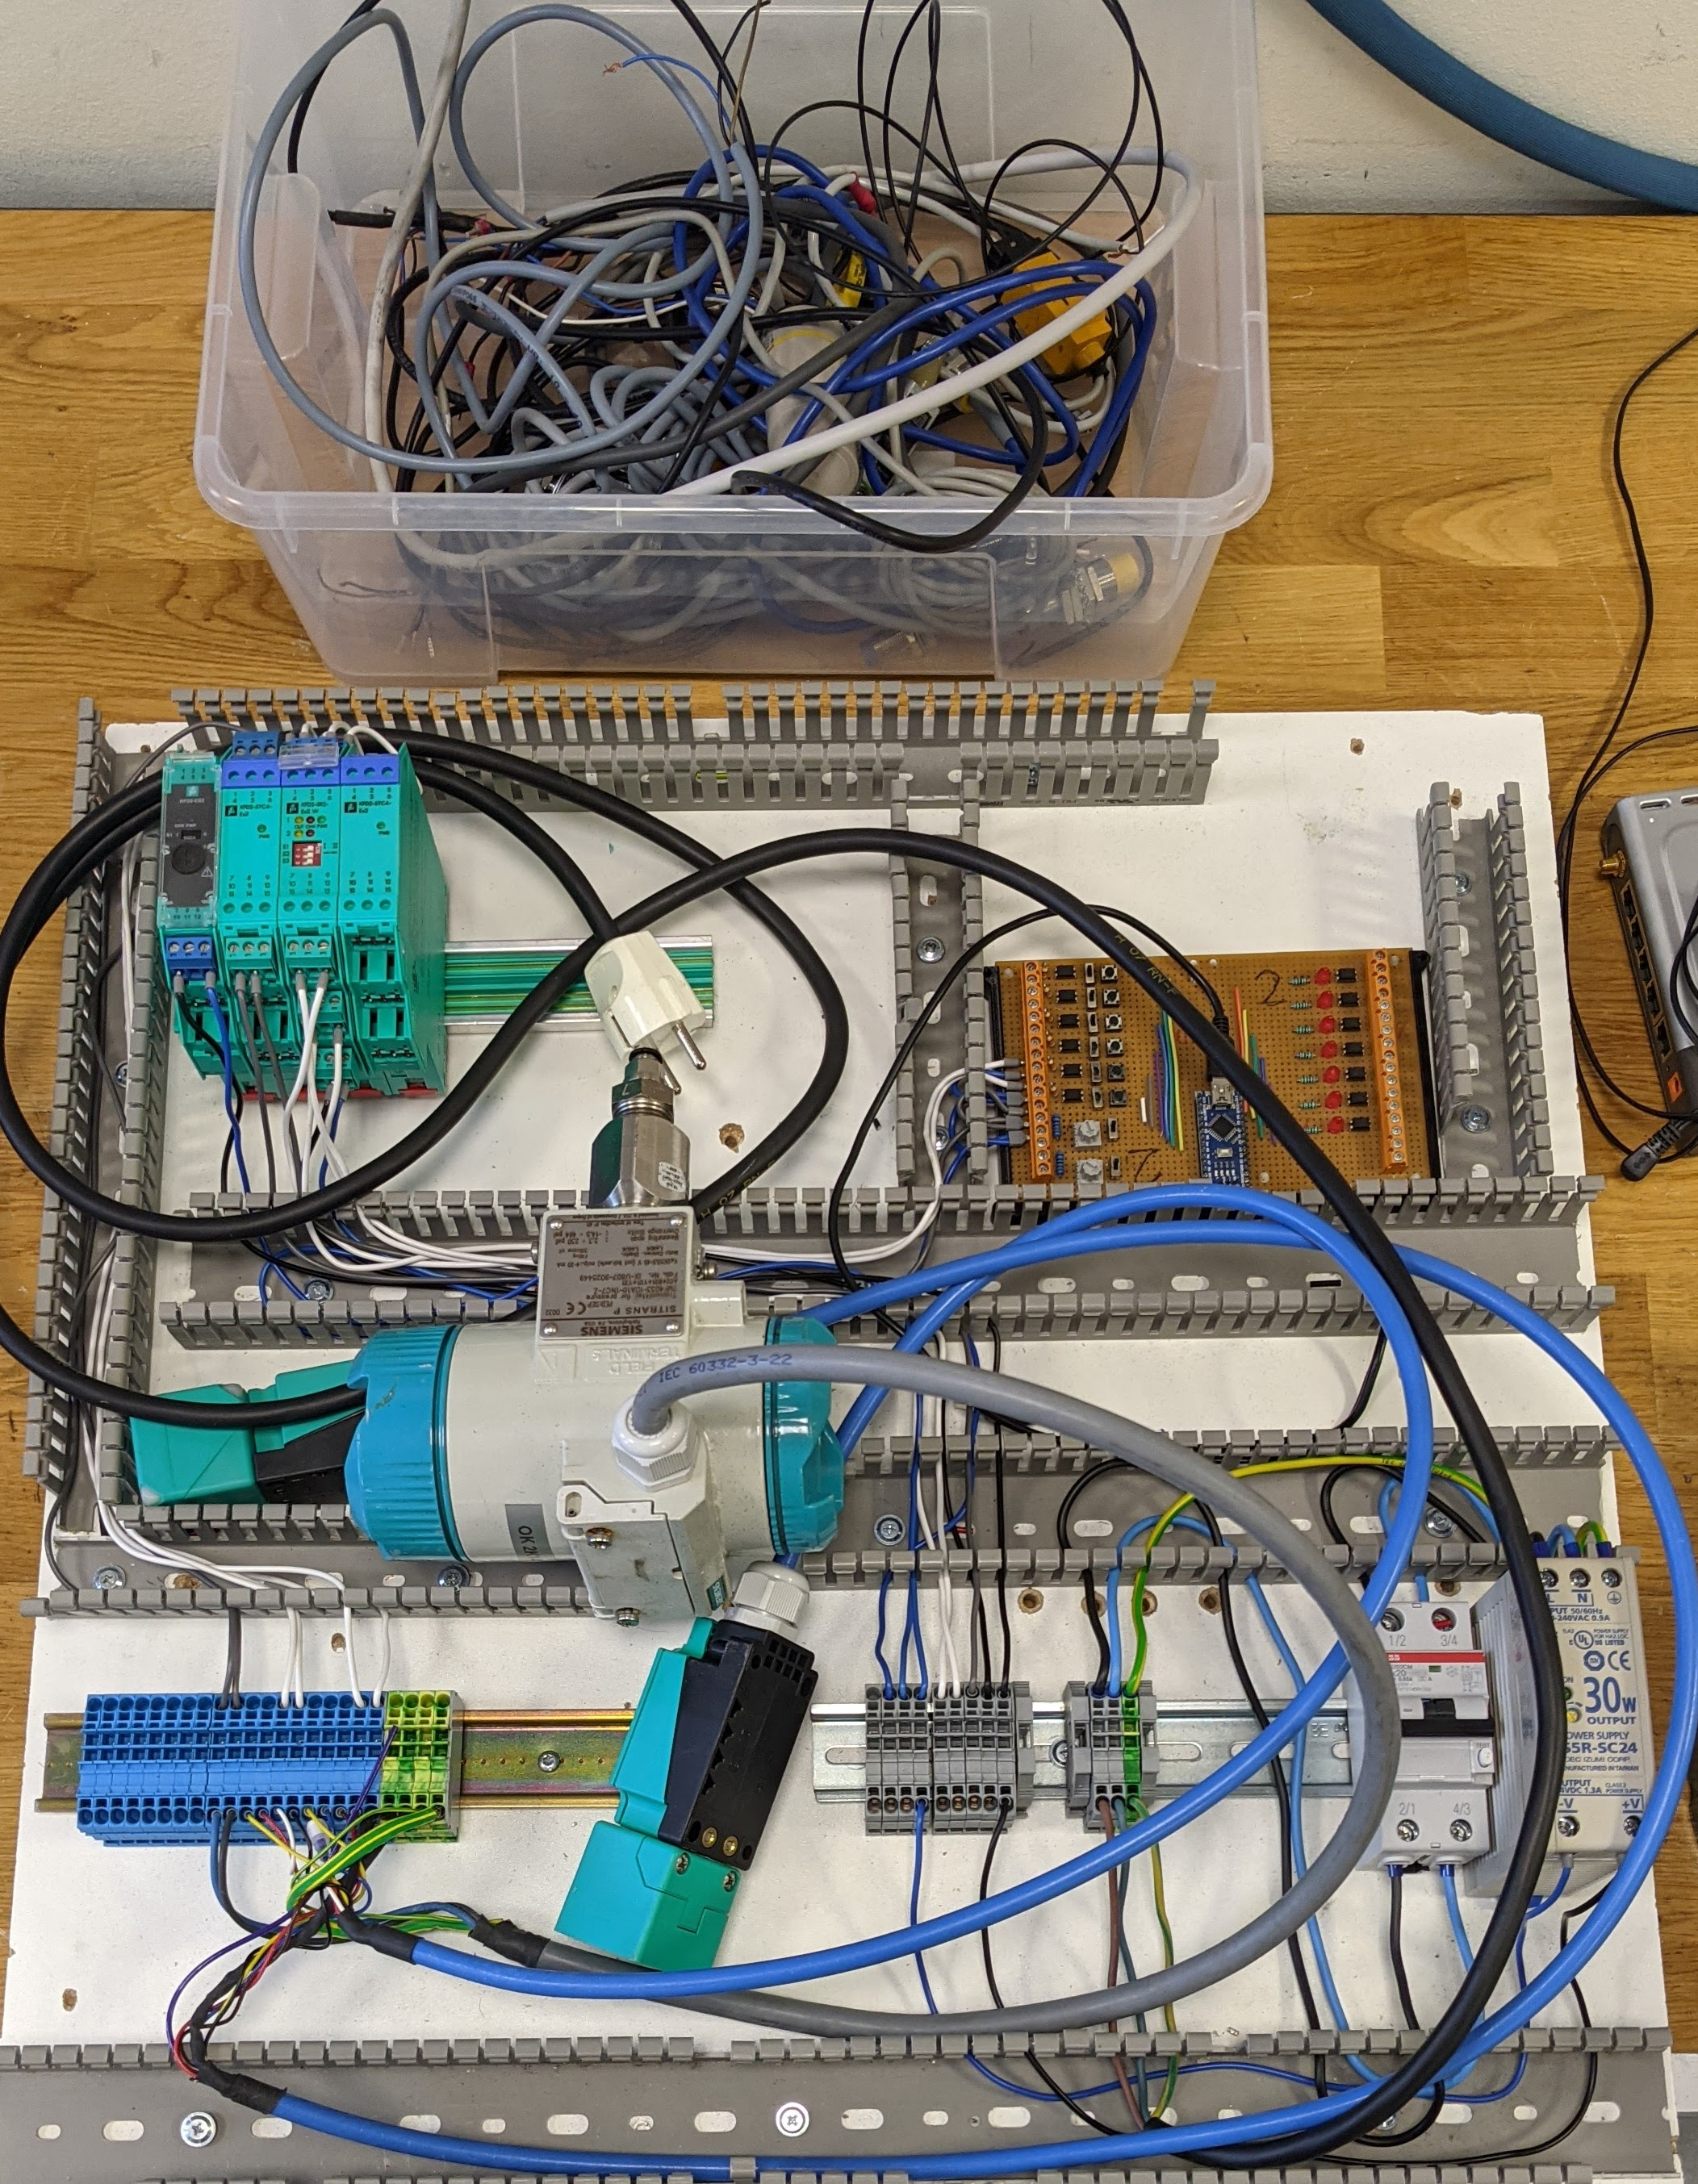
\includegraphics[width=13cm]{i04823x01.jpg}$$\\
\textbf{Kalibrering og justering range for en smart transmitter}
Målet med oppgaven er å lære hvordan vi justerer en transmitter for trykk.



\textbf{Arbidsoppdrag -- teorioppgaver}

\begin{enumerate}
	\item Sett deg inn i manualen til aktuell DP-celle
\end{enumerate}
\textbf{Arbidsoppdrag -- planlegging}

Utstyr:
\begin{itemize}[noitemsep]
	\item Trykktransmitter med HART kommunikasjon 
	\item Utstyr for å trykksette og å måle trykk 
	\item HART-communicator 
	\item +24VDC strømforsyning 
\end{itemize}

\textbf{Arbidsoppdrag -- gjennomføring}

Oppgaver\begin{enumerate}
	\item		Utført en As found kalibrering 
	\item		Bruk HART-communitatoren til å justere transmitteren slik at den gir 4 mA ved 1 barg og 20mA ved 6 barg 
	\item		Utfør en As left kalibrering 
\end{enumerate}
\textbf{Arbidsoppdrag -- dokumentasjon}

\begin{enumerate}
	\item Beskriv hvordan du planla, gjennomførte og dokumentere jobben. Forklar eventuelle avvik dere måtte observere under oppdraget. 
\end{enumerate}










\vfil 


\underbar{file i04843}
\vfil \eject
%(END_QUESTION)





%(BEGIN_ANSWER)


%(END_ANSWER)





%(BEGIN_NOTES)


%INDEX% Arbeisdoppdrag, Målesystemer, Nivå 1, Stasjon10, Kalibrering, DP-celle(Smart)

%(END_NOTES)


